\chapter{Parallelisation of exhaustive two-dimensional searches}
\label{Results2}
\lhead{Chapter 3. \emph{Parallelisation of exhaustive two-dimensional searches}}


\section{Abstract}
\setstretch{1}
A central problem with detecting epistasis is in overcoming the computational problems associated with a high dimensional search space. For example, the computational burden for a pairwise search of $p$ SNPs is $O(p(p-1)/2)$. The growing availability of multi-core personal computers, large scientific compute clusters, and massively multi-core consumer level graphics processing units (GPUs) now offer several avenues for the parallelisation of the search space, and for each of these architectures scalable software was written to distribute the workload of the search space. The CPU based architectures successfully scale almost linearly with the number of cores available, with relatively little modification of the serial algorithm required. For the GPU implementation, with recent hardware an increase in speed of two orders of magnitude against optimised serial code was achieved through substantial manipulation of the original algorithm. Ultimately, the software can be implemented cheaply to make exhaustive pairwise searches computationally tractable for dense SNP chips or even sequence data. The software is open source, platform independent, GPU vendor independent, and made freely available at \href{http://sourceforge.net/projects/epigpu}{http://sourceforge.net/projects/epigpu}.

\section{Introduction}
\setstretch{1.6}
Examination of the literature reveals an interesting disparity: the volume of work on the theoretical exploration of epistasis dwarfs the amount of actual empirical research performed, particularly in the context of human genetics. One of the major causes for this is likely to be the absence of reliable tools that will address the computational burden of expanding the search space from one dimension, as in traditional genome wide association studies, to two or more dimensions that are required to detect interactions. Stemming from this body of theoretical work, reviews on the subject have emerged periodically over the years (\emph{e.g.} \cite{Phillips1998, Cordell2002, Carlborg2004, Moore2005, Wagner2011}), largely advocating the inclusion of epistasis in complex trait analysis and its importance therein. However this enthusiasm is only very recently being matched with software that might make such analyses tractable, and of the recent releases most concentrate on binary traits, ignoring quantitative traits entirely. This chapter describes three new software implementations that have been written to parallelise a pairwise search on different types of hardware for quantitative traits.

\subsection{Computing hardware}

Computing performance in terms of processing speed and memory capacity are strongly dependent upon the number of transistors that can be integrated into a circuit. For several decades this number has doubled approximately every 18 months, a phenomenon known as Moore's Law \citep{Moore2006}. While Moore's law is expected to continue to be accurate for several more years, its relationship with processing speed is no longer holding. The abrupt departure from a historically exponential speed improvement is clearly shown in figure \ref{fig:clockspeed}. As transistor density increases the power required by the circuit increases also, such that inadequate heat dissipation leads to increased circuit resistance and instability. Cooling systems are not improving at a sufficient rate to nullify this problem, such that researchers can no longer simply wait for hardware improvements to abrogate their computationally intensive problems.

\begin{figure}
\begin{center}
\includegraphics[scale=0.7]{Chapter2/clockspeed.pdf}
\caption[CPU clockspeed changes over time]{Box and whisker plot showing progress in clock speed on a log scale, measured as millions of instructions per second (MIPS), over time in years. Data comprises processor speeds for Intel chips for most years since 1978, sourced from \cite{McKenney2011} and \href{http://csgillespie.wordpress.com/2011/01/25/cpu-and-gpu-trends-over-time/}{http://csgillespie.wordpress.com/2011/01/25/cpu-and-gpu-trends-over-time/}.
}
\label{fig:clockspeed}
\end{center}
\end{figure}


Because processing speed is unlikely to improve with current architectures, the alternative solution, which is in wide use today, is to use many processing cores in parallel. The expected speed improvement from this strategy is predicted using Amdahl's law \citep{Amdahl1967}, which defines $M$, the maximum speed-up obtained from parallelisation, as
\begin{equation}
\label{eq:amdahl}
M \leq \frac{1}{(1-P) + \frac{P}{C}}
\end{equation}
where $P$ is the proportion of the time of the serial programme that could be parallelised and $C$ is the number of cores across which the parallelisable section it is to be distributed. In the context of exhaustive pairwise searches for epistasis, $P \approx 1$ so the potential value of parallelisation is high.

The disadvantage of this strategy is that to harness the additional hardware performance often requires programmes to be restructured from the serial version significantly. Many different hardware architectures have been developed to enable parallelisation, but the three most widely used are multi-core CPUs, scientific compute clusters, and graphics cards. Multi-core CPUs mostly comprise two or four processing cores, with six cores recently becoming available also. Further, some motherboards can house two multi-core processors, so at most the speed improvement from this strategy is 12x faster than serial code.

Alternatively, at the cost of fast communication and shared memory between cores, Beowulf compute clusters scale the number of processing cores more economically by using many cheaper two- or four- core processors that communicate through ethernet. Many researchers have access to at least moderately sized clusters of this type.

Graphics cards have developed rapidly over the last decade and now incorporate hundreds of processing cores. GPU cores are much simpler than CPU cores, having been designed to simply calculate pixel colour values for graphical output, with little need for inter-core communication or sophisticated hardware implementations such as large memory cache or instruction controls. Nonetheless, many scientific computational problems are now being resolved through the various software implementations that enable `general purpose' graphics processing. Programming for these types of devices is, at the current stage of development, more challenging than writing efficient code for CPU architectures for several reasons. Most CPUs now have large memory caches (\emph{e.g.} $> 2MB)$ that are rapidly accessible by processing cores, but GPUs can only house their many cores by sacrificing these large memory caches, so memory management is critical. GPU kernels must be optimised manually because current kernel compilers are extremely primitive compared to their CPU counterparts. Also, with several hardware vendors using their own architectures, and older and newer versions of these architectures having different design features, making a programme that runs well on all graphics cards for all operating systems becomes difficult, forcing the programme to use the most generic hardware features in order to maintain compatibility. Yet despite these challenges some scientific computational problems have been alleviated effectively by GPUs, and in fact the most powerful supercomputers in the world are now designed to cluster many GPUs instead of CPUs, so this type of architecture is a natural candidate for parallelising epistatic scans.

\subsection{Currently available parallelised software}

For the purposes of genome-wide association studies, many software packages have been published and are made freely available, but they are almost exclusively concerned with independent locus effects. What follows over the next two sections is a brief summary of a number of colourfully named applications that are now making the search for epistasis a computational reality. Where timings for exhaustive scans are mentioned, they refer to the total time to search across 300000 SNPs comprising 1000 individuals, and where rates of tests per second are mentioned, it refers to the effective number of pairwise interactions for 1000 individuals.

One of the most widely used tools for GWAS, {\tt PLINK} \citep{Purcell2007}, has the option to perform exhaustive pairwise epistatic searches for both binary and quantitative traits. Yet, despite wide availability it is unlikely to be used due to prohibitive computational times. For example, because it evaluates approximately 5000 pairwise interactions per second, to perform an exhaustive pairwise search on 1000 individuals across 300,000 SNPs it would take approximately $\frac{300000 \times 299999 / 2}{5000 \times 60 \times 60 \times 24} \approx 200$ days. This increases to around 3 years for 1,000,000 SNPs. A more recent implementation called {\tt FastEpistasis} was implemented by \cite{Schupbach2010}, a module for which is now available on {\tt PLINK}, that both optimises the baseline code and parallelises across Beowulf clusters. This implementation parameterises the search for $additive + additive \times additive$ effects, and in serial can calculate approximately 36000 pairwise interactions per second, scaling linearly with the number of cores across which it is parallelised.

A few GPU implementations for binary traits have also become available recently. The parallelisation of a multifactor dimensionality reduction (MDR) scan \citep{Sinnott-Armstrong2009} was the first to appear in the literature, citing a 50x speed improvement against serial CPU code. However, its absolute speed still seems relatively slow, performing only 4100 pairwise interactions per second, making it unsuitable for dense SNP chips. Two more implementations that use a more traditional testing framework are also available, and they appear to be quite successful in achieving the kinds of speeds that would make analysis routinely possible. {\tt EPIBLASTER} \citep{Kam-Thong2010} operates in two stages, the first involves an exhaustive pairwise scan that screens for differences between Pearson correlations between cases and controls, this generates a small subset of potential interacting pairs that are then tested more rigorously using the more computationally expensive logistic regression calculation. This software performs approximately 1.5 million pairwise calculations per second, allowing the completion of an epistatic scan in approximately 24 hours. A second piece of software that uses a similar approach, {\tt SHEsisEPI} \citep{2050244420100701}, achieves a similar efficiency, completing a scan in 27 hours. All benchmarks were performed using a NVIDIA GeForce GTX295 GPU.


\subsection{Statistical approaches}

It is possible to avoid the brute force approach using feature selection methods, where the large set of parameters are filtered to make a small subset prior to the main analysis, such that although the dimensionality of the search space remains the same (two dimensional in this case), the magnitude of the dimensions are substantially reduced (here, offering a quadratic reduction in the search space, and therefore substantially reducing the multiple testing penalty also). Such methods have been investigated, but while being vastly superior in terms of computational time, exhaustive methods are generally more powerful \citep{Marchini2005, Evans2006}, and perhaps more importantly it can be demonstrated that replicating discoveries in different populations from filtered subsets is severely underpowered \citep{Greene2009}.

Alternative machine learning methods have also been suggested, but again these are largely tailored for binary phenotypes. An interesting idea is to use a support vector machine where formally the computational burden of a brute force search of $\sim O(p^2)$ is transformed to $\sim O(n^3)$, where $p$ is generally in the hundreds of thousands and $n$ is frequently several orders of magnitude smaller, however several approximations can be made to significantly reduce the formal complexity estimate (Bordwardt 2011?). A drawback of this approach is that the feature selection is restricted to a set of a few predefined functional genotype-phenotype maps, thus vastly reducing the scope of what can be detected. Another feature selection method, random forests, has been implemented as a generic library in R, {\tt R/randomForest}, and as an optimised version designed to search for two locus epistasis, {\tt Random Jungle} \citep{Schwarz2010}. This is an extremely fast approach, completing a scan within 13 hours. However it may not be suitable for a problem such as epistasis where the number of true features is extremely small relative to the high dimensionality of the search space \citep{Segal2004}. 

A non-parametric method, MDR, seeks to heuristically reduce the $3 \times 3$ contingency table for a binary phenotype to a set of two classes that is then scored by its prediction error from a $k$-fold cross validation. Though it has been used quite extensively for relatively sparse SNP panels it is computationally very intensive, and appears to be substantially less statistically efficient than traditional logistic regression approaches. Other approaches that involve improving the efficiency of brute force searches by approximating the standard likelihood ratio tests may be of greater efficacy. For example {\tt TEAM} \citep{Zhang2010} sidesteps the problem of generating test statistics, and instead approximates contingency tables for all pairwise SNPs through the use of minimum spanning trees derived from a small subset of the individuals in the sample. Another algorithm, {\tt BOOST} \citep{Wan2010}, approximates the conventional odds ratio test to a linear entropy model, which is then tested for divergence from linearity to indicate `synergistic' interactions, thereby reducing the test parameterisation to purely interaction terms. In doing so the model becomes faster to calculate, and further optimisation is achieved by bit-packing the data for low level CPU processing. 

With the brute force approach, as demonstrated in the few examples mentioned above there are numerous ways to parameterise a statistical test for pairwise epistasis, and there is no real consensus on what may be the `correct' approach. Classically, the genetic variance of the genotype-phenotype map can be partitioned into smaller components: $additive$, $dominance$, $additive \times additive$, $additive \times dominance$, $dominance \times dominance$, and higher order terms for higher dimensional interactions \citep{Cockerham1954, Jana1971}. {\tt FastEpistasis} limits the search to only include 3 degrees of freedom - $additive$ at both loci and $additive \times additive$ by performing a test of allelic association - however as demonstrated in chapter 2, these are the variance components that are least likely to persist over evolutionary time, so it may be premature to exclude other variance components at the genome scan stage. An alternative approach, as suggested by \cite{Cordell2002} and as used by {\tt EPIBLASTER}, is to base the statistical test only on interaction terms, excluding the marginal effects. While this specifically tests for epistasis, results from chapter 2 also show that this is substantially underpowered. Furthermore, with shifting allele frequencies between populations replication will again become problematic because the partitioning of variance components are likely to change significantly \citep{Greene2009}. 

\subsection{Summary}

Several potentially useful implementations exist for the epistatic analysis of binary phenotypes. However it is unclear how the various methods might compare to a traditional exhaustive search that performs a standard logistic regression. The approximation methods, {\tt BOOST} and {\tt TEAM}, ostensibly offer an extremely computationally efficient manner for exhaustive scans, but a rigorous investigation into a potential loss of statistical efficiency is warranted, and indeed this may not be viable yet with the GPU implementations also resorting to approximations instead of standard testing.

The approach that appears to be the most powerful for two dimensional searches is to test for whole pair genetic effects, as shown in chapter 2 and also supported by \cite{Marchini2005}. While a significant two-locus genetic effect does not necessarily constitute a significant epistatic effect, upon sequestering a set of candidate pairs from a genome wide scan the true contribution of epistasis can be assessed more rigorously. In any case, if the phenotype is corrected for large marginal effects prior to the epistatic scan it is unlikely that any candidate hits will be without epistasis. In summary, it appears it would be expedient to adhere to a policy of including all information for statistical efficiency, and implementing parallelisation methods for computational efficiency at this stage of our understanding. To this end, three programmes were developed that geometrically parallelise the exhaustive scan comprising linear regression against full pairwise genotype effects across desktop multi-core CPUs ({\tt episcan}), Beowulf clusters ({\tt epiMPI}), and consumer level GPUs ({\tt epiGPU}).


\section{Methods}

\subsection{Statistical tests}

All three programmes perform an exhaustive scan for pairwise interactions, such that each SNP is tested against all other SNPs for statistical association with the phenotype. Three different tests can be performed using the software, either treating the pairwise genotype classes as factor effects, parameterising the class means as only marginal effects, or parameterising the class means to exclude any marginal effects thus testing for only interaction terms.

There are 9 possible genotypes resulting from combining a pair of SNPs, assuming two alleles for each SNP. By treating the genotype classes as a fixed effect an 8 d.f. F-test can be performed that tests the following hypotheses:
\begin{equation}
H_{0}: \sum_{i=1}^{3}\sum_{j=1}^{3} (\bar{x}_{ij} - \bar{y})^{2} = 0; \label{eq:nullfull}
\end{equation}
\begin{equation}
H_{1}: \sum_{i=1}^{3}\sum_{j=1}^{3} (\bar{x}_{ij} - \bar{y})^{2} > 0; \label{eq:altfull}
\end{equation} where $\bar{y}$ is the phenotype mean and $\bar{x}_{ij}$ is the pairwise genotype class mean for genotype $i$ at locus A and genotype $j$ at locus B. This type of statistical test does not parameterise for specific types of epistasis, rather, it tests for the joint genetic effect at two loci.

The software is, however, capable of reducing the test to 4 d.f., parameterising for interaction terms only (\citealp{Cordell2002}). This is achieved by removing the marginal additive and dominance effects from each locus, testing the following hypotheses:
\begin{equation}
H_{0}: \sum_{i=1}^{3}\sum_{j=1}^{3} (\bar{x}_{ij} - \bar{x}_{i} - \bar{x}_{j} + \bar{y})^{2} = 0; \label{eq:nullint}
\end{equation}
\begin{equation}
H_{1}: \sum_{i=1}^{3}\sum_{j=1}^{3} (\bar{x}_{ij} - \bar{x}_{i} - \bar{x}_{j} + \bar{y})^{2} > 0; \label{eq:altint}
\end{equation} where $\bar{x}_i$ ($\bar{x}_j$) is the marginal class mean for genotype $i$ ($j$) at locus A (B).

Alternatively, there may be some reason to believe that when LD between causal variants and observed SNPs is low the interaction variance components shrink much faster than marginal components. Indeed, the marginal components may actually increase as they begin to capture some of the higher order components (see chapter 2). This can be parameterised as a 4 d.f. test using the following hypotheses:

\begin{equation}
H_{0}: \sum_{i=1}^{3}\sum_{j=1}^{3} (\bar{x}_{i} + \bar{x}_{j} - \bar{y})^{2} = 0; \label{eq:nullmarg}
\end{equation}
\begin{equation}
H_{1}: \sum_{i=1}^{3}\sum_{j=1}^{3} (\bar{x}_{i} + \bar{x}_{j} - \bar{y})^{2} > 0. \label{eq:altmarg}
\end{equation}

Because the computationally intensive aspect of the calculation is calculating the sums of squares it is possible to calculate all three parameterisations simultaneously with little memory or time cost relative to the calculation of the full parameterisation. The $F$ test is then performed as normal:

\begin{equation}
\label{eq:ftest}
F = \left(\frac{SS(model)}{d}\right)\left(\frac{SS(y) - SS(model)}{n-d-1}\right)^{-1} \sim F(d,n-d-1)
\end{equation}
where $d$ is the number of degrees of freedom, $n$ is the number of individuals, and $SS(model)$ is the sum of squares for a model parameterised as in equations (\ref{eq:nullfull}-\ref{eq:altmarg}), for example for equation (\ref{eq:nullfull})

\begin{equation}
SS(model) = \sum_{i=1}^{3}\sum_{j=1}^{3} n_{ij}(\bar{x}_{ij} - \bar{y})^{2}, \label{eq:ssfull}
\end{equation}
where $n_{ij}$ is number of individuals for the pairwise genotype class.

\subsection{Single node CPU optimisation}

The source for {\tt episcan} is written in ANSI C for ease of compilation on multiple platforms, computational efficiency, and extensibility. All benchmarking is performed on compilations made by GCC version 4.3.4, using -O2 optimisation controls.

Because the number of tests is likely to run into many billions, saving all test statistics is not convenient. For example, a 300k SNP chip where $F$ values are stored as single precision floating values will require $4.5 \times 10^{10} \times 32 / (1024^3) = 1341$ gigabytes of storage. Instead, the programme only stores the $F$ values from the scan that exceed a relatively low threshold. 

Most modern desktop computers and laptops have multi-core architectures. For parallelisation within a single node the OpenMP (open source multi-processing) specification was used. Briefly, the application programming interface (API), allows the programmer to use pre-processor directives, such that upon compilation the code is automatically refactored to distribute the work load across several threads. Usually the programme creates as many threads as there are processing cores, so that all cores are occupied continually. But on some more recent processors where hyperthreading is an option, each core can have two threads each, the advantage being that as a task from one thread is being processed, memory latencies can be eliminated on the other thread.

Specifically, for the main computational challenge of iterating through all pairwise $F$ values, where the programme is effectively populating the lower triangle of a $p \times p$ matrix (where $p$ is the number of SNPs), is parallelised using the OpenMP API. To facilitate memory concurrency the search grid is broken into rows, such that each thread's task is to perform all F tests for a row of the matrix. A queue of all $p-1$ tasks is created such that a new task is distributed to the next available thread.

{\tt episcan} can be directed to run in serial mode or parallel mode by the user.


\subsection{Multiple node CPU optimisation}

Because the parallelisation requires little communication between processors, distributing the workload across multiple nodes in a Beowulf cluster is relatively straightforward. The OpenMPI (open source message passing interface) API was used to write {\tt epiMPI} because of its availability on most scientific clusters. In order to make the distribution of work scale linearly with the number of cores available it is important to evenly balance the number of tests to be performed. This can be done in realtime, by using message passing to retrieve a work item in realtime, or by defining the section of the work grid that each node will perform prior to beginning the scan. Because the communication between nodes is relatively slow on most clusters, the latter approach was used.

\begin{algorithm}
\caption{Exhaustive pairwise search algorithm}
\label{algo:pairwise}
\begin{algorithmic}

\STATE $i:= b_i$
\FOR{$j := b_j$ to $b_i - 1$}
\STATE $F_{ij}:= f(y, x_i, x_j)$  \COMMENT{Beginning overhang}
\ENDFOR

\FOR{$i := b_i$ to $e_i - 1$}
\FOR{$j := 1$ to $i - 1$}
\STATE $F_{ij}:= f(y, x_i, x_j)$ \COMMENT{Body of scan}
\ENDFOR
\ENDFOR

\STATE $i:= e_i$
\FOR{$j := e_j$ to $e_i$}
\STATE $F_{ij}:= f(y, x_i, x_j)$ \COMMENT{Ending overhang}
\ENDFOR

\end{algorithmic}
\end{algorithm}

The total number of tests $T = p(p-1) / 2$ to be performed in an exhaustive pairwise search can be represented as in Algorithm \ref{algo:pairwise}, where $f(y, x_i, x_j)$ is the calculation of the $F$ value for the linear regression of SNP $x_i$ and SNP $x_j$ on the phenotype $y$, $i$ is the matrix row, $j$ is the matrix column, $b_{i(j)}$ is the matrix row (column) to begin the scan and $e_{i(j)}$ is the matrix row (column) to end the scan. 

For example to perform the scan in serial on a single core, $b_i := b_j := 1$ and $e_i := e_j := p$, such that the `overhang' sections of code can be ignored. However, to distribute across $c$ cores, each core must calculate its beginning and end coordinates within the matrix, and iterate through the rows in between. These coordinates can be calculated theoretically using Algorithm \ref{algo:triangular} where $C$ is the number of cores and $c$ is an identifier for an arbitrary core (in the range of $1...C$); and the function
\begin{equation}
g(c, C, p) = \lfloor 1 + \sqrt{1 + 8 \lfloor cp(p-1)/2C \rfloor} - k \rfloor \label{findi}
\end{equation}
where $k = 1$ if the square root value is an integer, or 0 otherwise, calculates the row position in the $F$ matrix; and the function
\begin{equation}
h(i, c, C, p) = \lfloor cp(p-1)/2C \rfloor - i(i-1)/2
\end{equation}
where, $\lfloor \cdot \rfloor$ takes the floor of the value, calculates the column position. However, while this is the most direct way of partitioning the search space, in practice this solution is not viable for realistic SNP densities because the floating point precision of most processors will not be sufficiently accurate to test if the square root value in equation (\ref{findi}) is an integer.

\begin{algorithm}
\caption{Theoretical balanced partitioning of triangular matrix across arbitrary number of cores}
\label{algo:triangular}
\begin{algorithmic}

% n(n-1)/2 = x
% n^2 - n - 2x = 0
% -b ÔøΩ sqrt(b^2 - 4ac) / 2a = n
% 1 + sqrt(1 + 8x) = 2n
% n = (1 + sqrt(1 + 8x) / 2

\IF {$c = 1$}
  \STATE $b_i := 1$
  \STATE $b_j := 1$
  \STATE $e_i := g(c, C, p) $
  \STATE $e_j := h(e_i, c, C, p) $

\ELSIF {$c = C$}
  \STATE $b_i := g(c-1, C, p)$
  \STATE $b_j := h(b_i, c, C, p)$
  \STATE $e_i := p$
  \STATE $e_j := p$

\ELSE
  \STATE $b_i := g(c-1, C, p)$
  \STATE $b_j := h(b_i, c, C, p)$
  \STATE $e_i := g(c, C, p) $
  \STATE $e_j := h(e_i, c, C, p) $
\ENDIF

  \IF{$b_i = (b_j+1)$}
    \STATE $b_i := b_i+1$
    \STATE $b_j := 1$
  \ELSE
    \STATE $b_j := b_j+1$
  \ENDIF

\end{algorithmic}
\end{algorithm}

To sidestep this problem, the original version of the programme approached the work load distribution from another approach and used a heuristic scheduling algorithm known as Longest Processing Time (LPT). This was simply accomplished by partitioning the search space into chromosome-by-chromsome scans, such that for 23 chromosomes there would be $23 \times (23+1) / 2 = 276$ blocks, and they could be distributed across the available cores. Naturally, chromosome lengths differ, and scanning the SNPs between chromosomes would create a rectangular work space while scanning the SNPs within chromosomes would create a triangular work space, ultimately creating a set of jobs with widely variable work sizes. LPT heuristically packs the cores with the work blocks in an efficient manner. It orders the blocks according to estimated processing time and then sequentially distributing the largest available block to the core with the smallest accumulated work size. Here the estimated processing time is simply the area of the work block. While this is a widely used approach, in the majority of situations it will be unable to perfectly distribute the work load across the cores. Indeed, it has been shown that the efficiency of LPT, in terms of trying to minimise the maximum partition size is at worst $\frac{4}{3}-\frac{1}{3C}$ times the optimal value \citep{Graham1969}.

\begin{figure}
\begin{center}
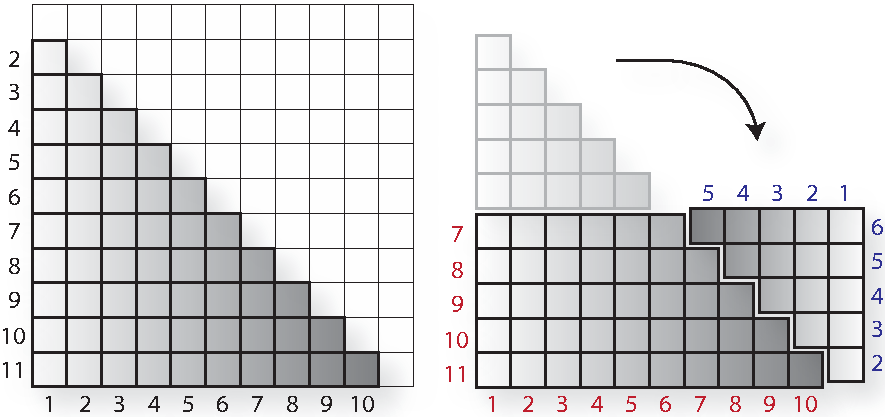
\includegraphics[width=4in]{Chapter2/tri_to_rect.pdf}
\caption[Distribution of triangular matrix work load]{Example of the recoding of the search space coordinates from a triangular to rectangular grid for efficient distribution across multi-core CPU clusters for 11 SNPs, as detailed in algorithm \ref{algo:rectangularisation}. The upper and lower triangular matrices are symmetrical, so only the shaded area is scanned (left). As the scan proceeds through the rectangular grid (right) iterating through rows $i = \{7,...,11\}$ and columns $j = \{1,...,11\}$. If $i > j$ then the SNPs tested are chosen according to the corresponding coordinates in red. If $i \leq j$ then the coordinates in blue are chosen.}
\label{fig:tri_to_rect}
\end{center}
\end{figure}


While the LPT achieves good efficiency, particularly with a very large number of available cores, it can be improved further. Here an alternative algorithm is devised that restructures the search grid to enable a computationally tractable and theoretically balanced work load across an arbitrary number of cores. First, the lower triangular matrix is partitioned into two sections by bisecting along the row $i = \lceil p / 2 \rceil$. By rotating the upper section (triangular matrix), and adjoining its diagonal with the diagonal on the lower section, a new rectangular matrix $R$ is created with dimensions $\lceil p / 2 \rceil$ rows and $p + l$ columns, where $l$ is 1 if $p$ is even, and $0$ otherwise (figure \ref{fig:tri_to_rect}).The search space is then simply distributed amongst cores by evenly partitioning the rows. Algorithm \ref{algo:rectangularisation} maps from the refactored rectangular matrix $R$ back to the coordinates of the original triangular matrix $F$, where the function
\begin{equation}
u(p, c, C) = \lceil cp/C(\lfloor p/2 \rfloor + 1) \rceil
\end{equation}
defines the row position of $R$. 

\begin{algorithm}
\caption{Rectangularisation and parallel distribution of triangular matrix}
\label{algo:rectangularisation}
\begin{algorithmic}

\IF{$c = 1$}
  \STATE $b_i := \lfloor p/2 \rfloor + 1$
  \STATE $e_i := u(p, c, C)$
\ELSIF{$c = C$}
  \STATE $b_i := u(p, c-1, C)+1$
  \STATE $e_i := p$
\ELSE
  \STATE $b_i := u(p, c-1, C)+1$
  \STATE $e_i := u(p, c, C)$
\ENDIF
\IF{$odd(p)$}
  \STATE $l := 1$
\ELSE
  \STATE $l := 0$
\ENDIF

\FOR{$i := b_i$ to $e_i$}
  \FOR{$j := 1$ to $p-l$}
    \IF{$j < i$}
      \STATE $F_{ij} := R_{ij} := f(y, x_i, x_j)$
    \ELSE
      \STATE ${i}' := p - i + 2 - l$
      \STATE ${j}' := p - j + 1 - l$
      \STATE $F_{{i}'{j}'} := R_{ij} := f(y, x_{{i}'}, x_{{j}'})$
    \ENDIF
  \ENDFOR
\ENDFOR

\end{algorithmic}
\end{algorithm}

\subsection{GPU optimisation}

The scan follows a single instruction-multiple data (SIMD) model, such that a fairly intensive kernel (the F test) is performed repeatedly on a large grid of data. The OpenCL (open source computing language) has been developed to allow multi-core architectures to generically parallelise such analyses. Of particular use is the ability of OpenCL to harness the massively multi-core architecture of modern graphics processing units (GPUs). Another such API, CUDA (compute unified device architecture), can also be used, however it is restricted to NVIDIA devices only. OpenCL was chosen for use in {\tt epiGPU} because it is open source and avoids the problem of being hardware vendor specific.

While most GPUs have hundreds of cores, performance doesn't necessarily scale proportionally, and not all algorithms will benefit from GPU parallelisation (\emph{e.g.} \citealp{Davis2011}). The main performance limiting factor is the memory input/output (I/O) bandwidth between processing cores and video memory. The computational kernel that runs on the GPU cores restructures the regression algorithm, making efficient use of the video memory hierarchies and this was necessary for achieving significant speed improvements. Several steps were necessary to limit the kernel I/O operations whilst maximising its efficiency, as outlined below.

\paragraph{Distribution strategy} The processing cores of the GPU are divided into groups of 8, known as streaming multiprocessors (SMs). These spawn and enqueue multiple threads for the execution of the kernel function, each thread being an F test for a different SNP pair. Ideally the number of threads per SM should be made as large as possible in order to minimise communications between CPU and GPU, and to reduce the number of kernel initialisations. However, for most operating systems the SM must not be occupied for more than 5 seconds (to allow other graphical devices to function), so the number of possible threads is restricted. The lower triangular $p \times p$ search grid must, therefore, be partitioned into a dense grid, such that each grid element can be sent to the GPU and executed within the allotted time.

\paragraph{Memory layout} GPUs partition their memory into four sections (in decreasing order of size, increasing order of speed): RAM, cache, local memory (L2), and private (L1). It is of primary importance to minimise time in piping data from various memory regions to the processing cores in order to achieve efficiency. The genotype data comprises the bulk of the information for performing the scan. This had to be mapped to the video random access memory (RAM), which is hierarchically the largest memory space but also the slowest to access. The phenotype is read only and, comprising a single vector of single precision floating point values, is stored in a smaller section of RAM that has faster access. Ideally this would be stored in L2 or L1 memory because it is accessed by every core for every F test, however these sections are extremely small, restricting this possibility. L2 and L1 share 16 kilobytes (kb) within each SM, effectively allowing 2kb per core. This was used to accrue the calculations for the nine genotype class means, $x_{ij}$, in $e.g.$ equation (\ref{eq:nullfull}) for each concurrent thread.

\paragraph{Use of on-line algorithms} Calculating the sum of squares of $y$ is conventionally done as
\begin{equation}
SS(y) = \sum^n (y - \bar{y})^2 \label{eq:ssy}
\end{equation}
where $n$ is the number of individuals. However, this would be problematic because of the requirement to first calculate the mean value of $y$ before being able to calculate its sum of squares. This isn't a problem when there are no missing values in the genotypes, because these values would not change, and they could be passed as precalculated values to the kernel. However, with missing values existing (as is often the case) an alternative method was devised. On-line algorithms are such that they can process the data incrementally in the order that the input is fed to them. In contrast, equation (\ref{eq:ssy}) is an off-line algorithm because it requires to have had access to all data prior to the calculation in order to calculate $\bar{y}$. This calculation was restructured to be made on-line based on \cite{Welford1962}, where $\bar{y}$ and $SS(y)$ for the entire cohort were passed to the kernel (calculated once for the whole scan on the CPU), and for every missing genotype value the individual's contribution was omitted according to Algorithm \ref{algo:on-line}, where the function $missing(X_{ik})$ tests if the $k$th individual's genotype at SNP $x_i$ is missing, and $\tilde{n}$ is the number of individuals with no missing genotypes for the pair of SNPs under test.

\begin{algorithm}
\caption{On-line algorithm for updating $SS(y)$ and $\bar{y}$}
\label{algo:on-line}
\begin{algorithmic}

\STATE $\tilde{n} := n$
\STATE $\tilde{SS(y)} := SS(y)$
\STATE $\tilde{\bar{y}} := \bar{y}$
\FOR{$k := 1$ to $n$}
\IF{$missing(X_{ik}) \cup missing(X_{jk})$}
\STATE $\tilde{SS(y)} := \tilde{SS(y)} - (y_k - \tilde{\bar{y}})(y_k - (\tilde{n}\tilde{\bar{y}} - y_k)/(\tilde{n}-1))$
\STATE $\tilde{\bar{y}} := (\tilde{n}\tilde{\bar{y}} - y_k)/(\tilde{n}-1)$
\STATE $\tilde{n} := \tilde{n} - 1$
\ENDIF
\ENDFOR

\end{algorithmic}
\end{algorithm}


\paragraph{Vectorising phenotype reads} The two major hardware vendors of graphics cards, ATI and NVIDIA, have both implemented hardware level vectorisation capabilities. Theoretically this means that 4, 8 or 16 array elements can be fetched from video RAM to L2 memory in the time that fetching a single array element would take using the non-vector form. These memory channels were used to read the phenotype values by the kernel.

\paragraph{Bit-packing genotype data} Each genotype is encoded as 0, 1, 2 to denote the number of minor alleles, or 3 to denote a missing value. Therefore only two bits are required to store a single genotype, such that even by storing them as $char$ data types, the smallest native data type in ANSI C at 8 bits, is relatively wasteful of bandwidth when the kernel fetches the data from RAM to L2. A beneficial trade-off could be made whereby encoding the genotype array to bit-pack 16 genotypes into an $int$ data type (32 bits) would increase transfer rates sufficiently even with the small cost of the kernel having to unpack the data upon its arrival for processing. For example, say the genotypes for an individual are $\{0, 1, 2, missing\}$, when encoded as normal, using an array of $char$ data types this would be stored as $\{ 00000000, 00000001, 00000010, 00000011 \}$, but the corresponding encoding when bit-packed would be a single $char$ element comprising the last two bits of each array element, $\{ 00011011 \}$. Another obvious benefit is that the genotype data requires much less space in video RAM, so even extremely large datasets could be comfortably accommodated on most GPUs.


\section{Results}

The software produced geometrically parallelises exhaustive searches for pairwise epistatic associations with quantitative traits. Large scale analyses were performed on simulated data, typical in scale of those that would be expected based on GWASs already published, on several different software and hardware systems. The performance tests show that against the baseline system (serial code running on a modern CPU) graphics cards can perform the same analysis almost two orders of magnitude faster and at minimal expense (Table~\ref{tab:parallel}), such that an analysis that would take over 4 days to complete using {\tt episcan} in serial mode could be performed in just over an hour by using software utilising a graphics card. It is demonstrable that to achieve comparable speeds using CPU cores would require a large compute cluster, for which the cost to acquire and administer could be prohibitively expensive.

Compared to existing software, these implementations appear to perform favourably. Comparing {\tt episcan} against {\tt FastEpistasis}, both running in serial, {\tt episcan} runs approximately $3.5\times$ faster, performing $128200$ tests per second. Both programmes scale almost linearly with the number of cores. {\tt EPIBLASTER} is the most efficient GPU based implementation currently available, and {\tt epiGPU} (using the values from the Nv GTX285, a similar card to the one used by \cite{Kam-Thong2010}) performs almost $4 \times$ faster in terms of tests per second.

\renewcommand{\arraystretch}{1.2}
\begin{table}[!t]
\rowcolors{3}{tableShade}{white}
\begin{threeparttable}
\caption{\label{tab:parallel}Parallelisation performance and cost comparison}
\begin{tabular}{llrrrr} \toprule 
Parallelisation & Hardware & \multicolumn{1}{c}{Cost} & \multicolumn{1}{c}{Time} & \multicolumn{1}{c}{Relative} & \multicolumn{1}{c}{Cost} \\
& & \multicolumn{1}{c}{/ \textsterling \tnote{d}} & \multicolumn{1}{c}{/ min \tnote{e}} & \multicolumn{1}{c}{Speed \tnote{f}} & \multicolumn{1}{c}{benefit \tnote{g}}\\ \toprule
None 	& Baseline CPU \tnote{a} & - & 5860 & 1.0 & -\\
%& & & & \\
%\midrule
Multi-core CPU	& 6-core CPU \tnote{b} & 760 & 986 & 5.9 & 1.6\\
		& 8-core CPU \tnote{c} & 1600 & 763 & 7.7 & 1.0\\ 
%& & & & \\
%\midrule
CPU cluster \tnote{c}	& 16-core cluster & - & 398 & 14.7 & -\\ 
		& 32-core cluster & - & 195 & 30.0 & -\\ \
		& 64-core cluster & - & 96 & 61.0 & -\\ 
%& & & & \\
%\midrule
GPU	& Nv Fermi GTX580 & 367 & 63 & 91.6 & 51.9\\
		& ATI Radeon 6970 & 300 & 86 & 68.1 & 47.2\\
		& Nv Tesla S1070 & 960 & 146 & 40.1 & 9.0\\
		& Nv GTX285 & 230 & 145 & 40.1 & 36.2\\
		& Nv 8800GT & 72 & 613 & 9.6 & 27.7\\ \bottomrule
\end{tabular}
\begin{tablenotes}{\footnotesize
\item[a] Baseline equipment, Intel i7 970 3.2GHz, running in serial
\item[b] Intel i7 970 3.2GHz
\item[c] Dual Intel Xeon E5472 3.0GHz
\item[d] Approximate cost for equipment above baseline. Cost estimates for large compute clusters are too subjective for realistic comparisons
\item[e] Total user time to complete the analysis (300,000 SNPs, 1000 individuals)
\item[f] Time relative to baseline time
\item[g] Cost benefit calculated as Speed / Cost, figures shown are adjusted relative to the cost of the best performing desktop CPU alternative (8-cores).}
\end{tablenotes}
\end{threeparttable}
\end{table}

The use of graphics cards as tools for scientific research is a rapidly emerging industry that has manifested staggering improvements in performance over the last few years. However it is still in its infancy, and as reflected in figure \ref{fig:gpuoptimisation}, the level of manual optimisation required by developers to harness this power is considerable. Furthermore, while a very heterogeneous array of devices can be used for OpenCL applications, differences in their architectures inevitably results in different responses to optimisation strategies. Figure \ref{fig:gpuoptimisation} shows that without careful optimisation, even the most recent GPUs will appear to offer little to no advantage over CPU implementations.

\begin{figure}
\begin{center}
\includegraphics[scale=0.7]{Chapter2/gpuoptimisation.pdf}
\caption[Assessment of GPU optimisation techniques]{Incremental improvements in performance by incorporating different GPU optimisation methods. For reference, the CPU speeds for {\tt episcan} are shown as horizontal lines (serial and parallelised on Dual socket Intel Xeon E5472). Speeds are for calculating 8 d.f. F tests with 1000 individuals.}
\label{fig:gpuoptimisation}
\end{center}
\end{figure}


\section{Discussion}

Quantitative genetics has long been occupied with the theoretical contribution of genetic variants to complex traits. The last decade has seen a global effort to start investigating this empirically on a large scale, yet epistasis remains largely unexplored. Computing exhaustive pairwise epistatic scans is an important step in making tractable the understanding of non-additive genetic effects in complex traits. Shown in this study, this can be achieved efficiently by using consumer level graphics cards, an established technology that is cheap and widely available. In its current implementation, {\tt epiGPU} is limited to performing linear regression on quantitative traits, but the parallel decomposition framework is sufficiently generic to allow its extension to other pairwise statistical analyses relatively easily, such as Chi-square testing for case-control data.

Another central problem with epistasis scans is the heavy multiple testing penalty incurred by stringent significance thresholds. Computationally straightforward methods such as the Bonferroni correction are likely to penalise for an overestimated number of independent tests, and this is particularly problematic with epistasis where the dimensionality of the search is increased. However, with the growing availability of GPU clusters (\citealp{Fan:2004:GCH:1048933.1049991}), it is now becoming feasible to perform two-dimensional genome-wide permutation analyses to generate more accurate estimates of family-wise false discovery rates (\citealp{Churchill1994a}), a potentially critical step toward understanding the contribution of epistasis towards complex traits.

It should also be noted that there is no consensus on how traditional brute force techniques might compare against the emerging machine learning methods, based on techniques such as random forests or support vector machines. To effectively evaluate statistical performances of these methods, computational problems must be minimised in order to perform meaningful simulations and to generate accurate family wise false discovery rates.


